\documentclass[12pt]{article}
\newif\ifanswer%\answertrue% comment out \answertrue to show/hide answers
\usepackage{../../preamble}% preamble always after \newif\ifanswer
%\pagenumbering{gobble}
\title{MathCounts East San Gabriel Valley Chapter, February 2021 \\ Target Round}
\author{Patrick \& James Toche}
\date{Revised:~\today}

\begin{document}
\maketitle
\begin{minipage}{\textwidth}
\begin{abstract}\setlength{\parindent}{0pt}%
Notes on Target Round of MathCounts East San Gabriel Valley Chapter Competition, February 2021. 
Questions are from MathCounts Foundation (\url{https://www.mathcounts.org/}). Copyright restrictions may apply. Written for personal use. 
Please report typos and errors over at \url{https://github.com/ptoche/Math/tree/master/mathcounts}. 
\end{abstract}
\end{minipage}

\thispagestyle{empty}
\clearpage

\section*{Target Round}


%%%%%%%%%%%%%%%%%%%%%%%%%%%%%%%%%%%%%%%%%%%%%%%%%%%%%%%%%%%%%%%%%%%%%%%%
\subsection*{1.}
If there are $0.624782$ lugs in a pique, then how many piques are in $200$ lugs? Express your answer to the nearest integer.

\nopagebreak

\fbox{\phantom{ANSWER}}~piques

\nopagebreak

\begin{answer}
$0.624782$ is to $1$ as $200$ is to $x$:
\begin{align*}
x = \frac{200}{0.624782} 
  = 320.1117
  \approx 320
\end{align*}
\begin{empheq}[box={\mathbox[colback=white]}]{equation*}
    320 ~\text{piques}
\end{empheq} 
\end{answer}
%%%%%%%%%%%%%%%%%%%%%%%%%%%%%%%%%%%%%%%%%%%%%%%%%%%%%%%%%%%%%%%%%%%%%%%%

\iftoggle{showAnswers}{\newpage}

%%%%%%%%%%%%%%%%%%%%%%%%%%%%%%%%%%%%%%%%%%%%%%%%%%%%%%%%%%%%%%%%%%%%%%%%
\subsection*{2.}
Consecutive integers are arranged in three columns in the pattern shown. What number will appear in column C in row $22$?

\nopagebreak

\begin{center}
    \rowcolors{2}{white}{gray!20}
\begin{tabular}{@{}C{2cm}C{2cm}C{2cm}L{3cm}@{}} 
          A &        B &        C & \\
          1 &        2 &        3 & row 1\\
          6 &        5 &        4 & row 2\\
          7 &        8 &        9 & row 3\\
         12 &       11 &       10 & row 4\\
         13 & $\vdots$ & $\vdots$ & row 5\\
   $\vdots$ & $\vdots$ & $\vdots$ & $\vdots$
\end{tabular}
\end{center}

\nopagebreak

\fbox{\phantom{ANSWER}}

\begin{answer}
This is a `boustrophedon' arrangement. We are interested in an even row, so we can start from the second row and ignore the `boustrophedon' arrangement by focusing on even rows only. 
\begin{center}
\begin{tabular}{@{}C{3cm}C{2cm}@{}} 
   Row number & Column C \\
            2 &        4 \\
            4 &       10 \\
            6 &       16 \\
     $\vdots$ & $\vdots$ \\
\end{tabular}
\end{center}
This is an arithmetic sequence with common difference $6$. For even terms, we have
\begin{align*}
S_{2n} = 4 + 6(n-1) \Rightarrow S_{22} = 4 + 6 (11-1) = 64
\end{align*}
\begin{empheq}[box={\mathbox[colback=white]}]{equation*}
    64
\end{empheq} 
\end{answer}
%%%%%%%%%%%%%%%%%%%%%%%%%%%%%%%%%%%%%%%%%%%%%%%%%%%%%%%%%%%%%%%%%%%%%%%%

\iftoggle{showAnswers}{\newpage}

%%%%%%%%%%%%%%%%%%%%%%%%%%%%%%%%%%%%%%%%%%%%%%%%%%%%%%%%%%%%%%%%%%%%%%%%
\subsection*{3.}
Jamie makes $120$ slices of toast and puts at most one spread (jam, butter or avocado) on each slice. She puts jam on $\dfrac{1}{3}$ of the slices, butter on $15$ of the slices and avocado on $50\%$ of the slices. How many slices of Jamie's toast have no spread?

\nopagebreak

\fbox{\phantom{ANSWER}}~slices

\nopagebreak

\begin{answer}
Let $j$, $b$ and $a$ stand for `jam', `butter', `avocado', and $x$ stand for `no spread'. The question statement implies:
\begin{align*}
j & = \frac{1}{3} (j+b+a+x) \\
b & = 15 \\
a & = \frac{1}{2} (j+b+a+x) \\
j+b+a+x & = 120
\end{align*}
From the first and third equation, $3j=2a$, which may be substituted into the first equation, so that all things considered:
\begin{align*}
j & = 40 \\
b & = 15 \\
a & = 60 \\
40 + 15 + 60 + x & = 120
\end{align*}
which yields $x=5$.
\begin{empheq}[box={\mathbox[colback=white]}]{equation*}
    5 ~\text{slices}
\end{empheq} 
\end{answer}
%%%%%%%%%%%%%%%%%%%%%%%%%%%%%%%%%%%%%%%%%%%%%%%%%%%%%%%%%%%%%%%%%%%%%%%%

\iftoggle{showAnswers}{\newpage}

%%%%%%%%%%%%%%%%%%%%%%%%%%%%%%%%%%%%%%%%%%%%%%%%%%%%%%%%%%%%%%%%%%%%%%%%
\subsection*{4.}
Segment $AB$ is $2808$ units long. Point $X$ is the midpoint of segment $AB$. Point $R$ is $\dfrac{3}{4}$ of the way from $X$ to $B$. Point $S$ is $\dfrac{5}{9}$ of the way from $X$ to $R$. How many units long is segment $RS$?

\nopagebreak

\fbox{\phantom{ANSWER}}~units

\nopagebreak

\begin{answer}
It pays to draw a picture.
\begin{center}
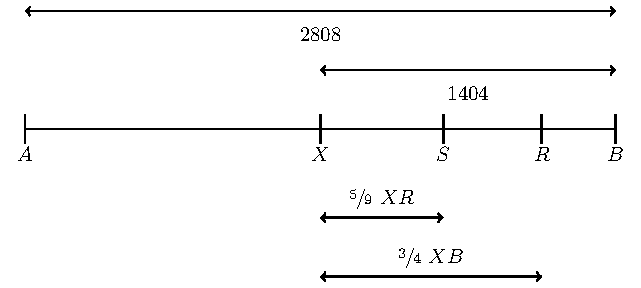
\includegraphics[height=6cm]{target-04-figure}
\end{center}
The distance from $X$ to $R$ is:
\begin{align*}
\frac{3}{4} \times \frac{2808}{2} = 1053
\end{align*}
The distance from $X$ to $S$ is:
\begin{align*}
\frac{5}{9} \times 1053 = 585
\end{align*}
The length of segment $RS$ is equal to the difference between $XR$ and $XS$:
\begin{align*}
1053 - 585 = 468
\end{align*}
\begin{empheq}[box={\mathbox[colback=white]}]{equation*}
    468 ~\text{units}
\end{empheq} 
\end{answer}
%%%%%%%%%%%%%%%%%%%%%%%%%%%%%%%%%%%%%%%%%%%%%%%%%%%%%%%%%%%%%%%%%%%%%%%%

\iftoggle{showAnswers}{\newpage}

%%%%%%%%%%%%%%%%%%%%%%%%%%%%%%%%%%%%%%%%%%%%%%%%%%%%%%%%%%%%%%%%%%%%%%%%
\subsection*{5.}
Twenty toothpicks, each $6$cm long, form a figure consisting of six equilateral triangles and a rectangle as shown. What is the total area of the figure? Express your answer as a decimal to the nearest hundredth.

\begin{center}
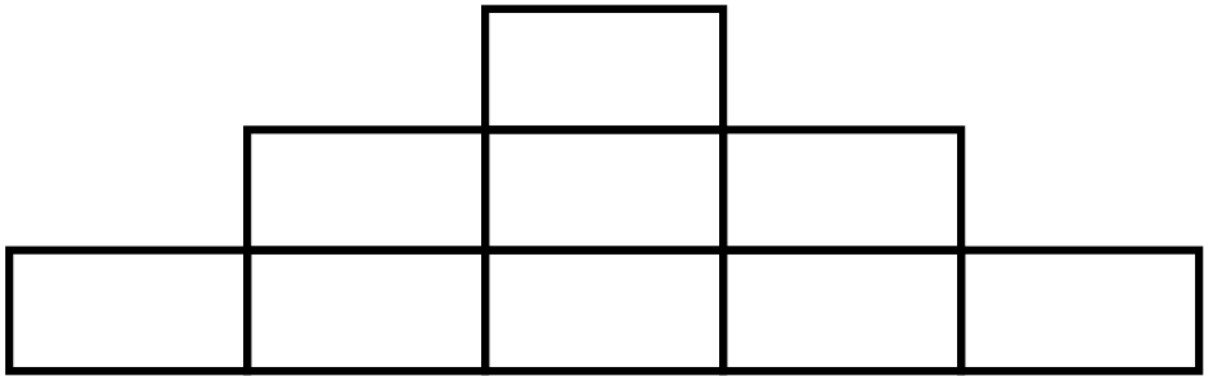
\includegraphics[height=6cm,page=1]{target-05-figure}
\end{center}

\nopagebreak

\fbox{\phantom{ANSWER}}~cm$^2$

\begin{answer}
The area of the central rectangle is $3$ times the area of a square with side length $6$\,cm, or $108$\,cm$^2$. The area of one triangle is equal to $3h$ (one-half of the product of the base $6$ and height $h$), where the height $h$ can be calculated by the Pythagoras theorem, as follows. Split the triangle vertically down the middle into two halves. Thus,the hypotenuse has length $6$ and the known leg has length $3$, as shown:
\begin{center}
\includegraphics[height=6cm,page=2]{target-05-figure}
\end{center}
We have
\begin{align*}
h^2 + 3^2 & = 6^2 \\
\Rightarrow h & = \sqrt{36-9} = 3\sqrt{3}
\end{align*}
The total area is therefore
\begin{align*}
3 \times 6^2 + 6 \times 3 \times 3\sqrt{3} 
  = 108 + 54\sqrt{3})
\approx 201.53
\end{align*}
\begin{empheq}[box={\mathbox[colback=white]}]{equation*}
    201.53 ~\text{cm}^2
\end{empheq} 
\end{answer}
%%%%%%%%%%%%%%%%%%%%%%%%%%%%%%%%%%%%%%%%%%%%%%%%%%%%%%%%%%%%%%%%%%%%%%%%

\iftoggle{showAnswers}{\newpage}

%%%%%%%%%%%%%%%%%%%%%%%%%%%%%%%%%%%%%%%%%%%%%%%%%%%%%%%%%%%%%%%%%%%%%%%%
\subsection*{6.}
There are $10$ coins on a table heads side up. Noah wants them all to be tails side up, but with each move, he must turn over exactly $6$ coins. What is the fewest moves he can take so that he ends up with all of the coins tails side up?

\nopagebreak

\fbox{\phantom{ANSWER}}~moves

\begin{answer}
To get a handle on this problem, consider some simple examples. Things get interesting after the second flipping. It is obvious that coins that were flipped at the first round from $H$ to $T$ will now be flipped back to $H$. It is also obvious that we exercise some control over how many coins will be flipped. Below we show several possibilities for the second move. In Move $\#2a$, we grabbed all four $H$ coins, together with two $T$ coins, with the result that two $H$ coins remain. In Move $\#2b$, we grabbed three of the four $H$ coins, together with three $T$ coins, with the result that four $H$ coins remain. It is clear that at this stage there can be $2$, $4$, $6$, and $8$ $H$ coins (this last case returns to the initial state and is not shown). And now a solution pops up: After Move $\#2c$, there are six $H$ coins that may be flipped to $T$ on the third (and last) move. 
\begin{center}
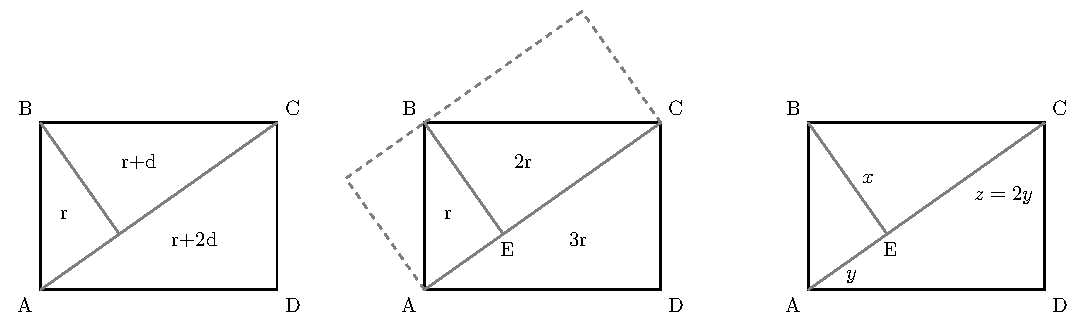
\includegraphics[height=6cm]{target-06-figure}
\end{center}
\begin{empheq}[box={\mathbox[colback=white]}]{equation*}
    3 ~\text{moves}
\end{empheq} 
\end{answer}
%%%%%%%%%%%%%%%%%%%%%%%%%%%%%%%%%%%%%%%%%%%%%%%%%%%%%%%%%%%%%%%%%%%%%%%%

\iftoggle{showAnswers}{\newpage}

%%%%%%%%%%%%%%%%%%%%%%%%%%%%%%%%%%%%%%%%%%%%%%%%%%%%%%%%%%%%%%%%%%%%%%%%
\subsection*{7.}
Suppose that $n$ is a positive integer for which the product $35n$ is divisible by $60$. What is the least possible value of $n$?

\nopagebreak

\fbox{\phantom{ANSWER}}

\begin{answer}
The factors of $35$ are $5$ and $7$, of which only $5$ is a factor of $60$, with $60=5\times12$, so that $n=12$:
\begin{align*}
35n & = 5 \times 7 \times n \\
    & = 5 \times 7 \times 12 \\
    & = 7 \times 60
\end{align*}
\begin{empheq}[box={\mathbox[colback=white]}]{equation*}
    12
\end{empheq} 
\end{answer}
%%%%%%%%%%%%%%%%%%%%%%%%%%%%%%%%%%%%%%%%%%%%%%%%%%%%%%%%%%%%%%%%%%%%%%%%

\iftoggle{showAnswers}{\newpage}

%%%%%%%%%%%%%%%%%%%%%%%%%%%%%%%%%%%%%%%%%%%%%%%%%%%%%%%%%%%%%%%%%%%%%%%%
\subsection*{8.}
Tim has a collection of square tiles of various sizes, each of which has an etched quarter circle with radius equal to the side length of the tile. Tim arranges eight tiles as shown. If the two smallest tiles each have side length $10$cm, what is the length of the resulting spiral formed by the tiles' etchings? Express your answer in terms of $\pi$?

\begin{center}
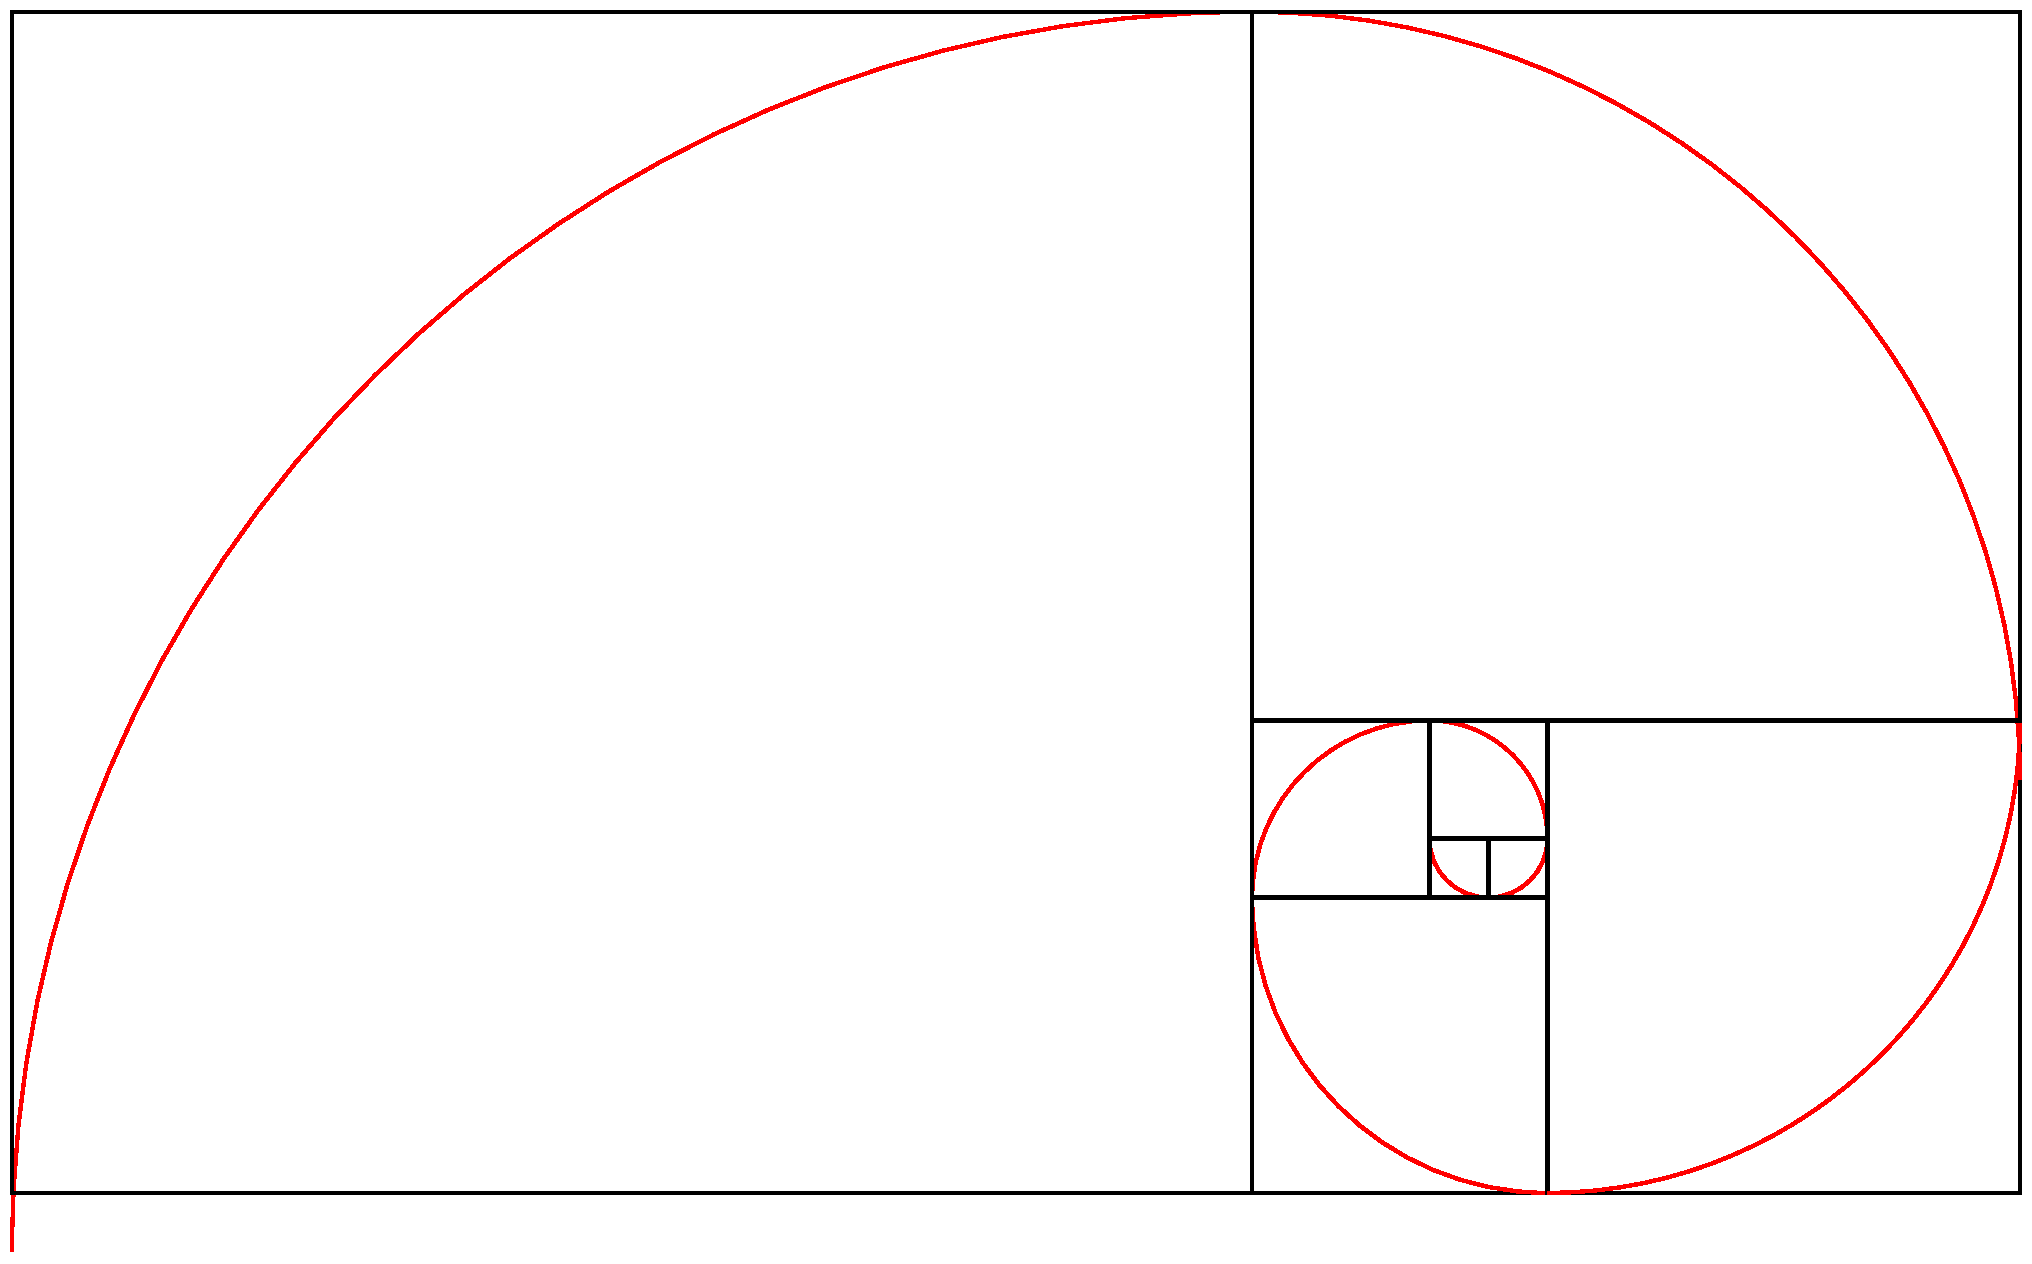
\includegraphics[height=6cm]{target-08-figure}
\end{center}

\nopagebreak

\fbox{\phantom{ANSWER}}~cm

\begin{answer}
Consider any square. Its side is also the radius of that portion of the spiral inscribed in it, which spans a quarter-circle. The length of the quarter-circle is $r\pi/2$, where $r$ is the length of the square's side. The total length of the spiral is the sum of the eight quarter-circles. But what are the side lengths of these squares? We recognize the Fibonacci pattern: The side of the largest square has length equal to the sum of the two smaller squares next to it. And this pattern holds for all squares except the squares in the center of the figure. Thus, the Fibonacci sequence starts with the two central squares at the center and grows outwards. The standard Fibonacci sequence is obtained by adding two consecutive terms in the sequence to obtain the next, starting with initial values $1$, and $1$. Thus,
\begin{align*}
1, 1, 2, 3, 5, 8, 13, 21
\end{align*} 
However, here, instead of $1$ and $1$, the starting values are $10$ and $10$. It is apparent that the modified sequence is simply scaled up by a factor of $10$:
\begin{align*}
10, 10, 20, 30, 50, 80, 130, 210
\end{align*}
Starting from the smallest square and going up:
\begin{align*}
\left(10+10+20+30+50+80+130+210\right)\pi/2
= 270 \pi
\end{align*}
\begin{empheq}[box={\mathbox[colback=white]}]{equation*}
    270\pi ~\text{cm}
\end{empheq} 
\end{answer}
%%%%%%%%%%%%%%%%%%%%%%%%%%%%%%%%%%%%%%%%%%%%%%%%%%%%%%%%%%%%%%%%%%%%%%%%


\end{document}